\section{Planned state of the application} The main reason for creating a new application instead of refactoring the current one is a change in the application's architecture. A new modernized architectural design of the BI-DBS portal was composed by Ing. Andrii Plyskach in his master thesis\cite{mt-plyskach}. We are aiming to correct all the mistakes made in the current application. It is essential to ascertain that we have chosen the right stack of technologies according to the newly chosen architecture.

\subsection{Architecture}
Microservices architectural pattern\cite{architecture-haris} is based on the concept of a series of loosely-coupled services. They can be developed using different technologies and deployed independently. It is more complex architecture than a standard monolithic one. You can see the diagram illustrating microservices architecture in Figure 1.2. 

\begin{figure}[hp]
\centering
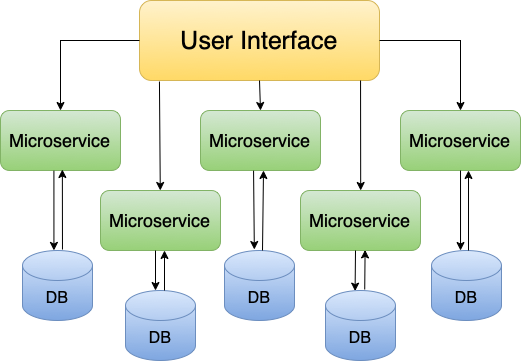
\includegraphics[scale=0.67]{../png/microservices.png}
\caption{Microservice architecture}\label{picture:microservices}
\end{figure}


\paragraph*{Advantages:}
\begin{itemize}
  \item \emph{Code readability:} When services are not strongly dependent the code appears to be better structured and easier to understand, which is a significant benefit for the BI-DBS portal.
  
  \item \emph{Independency in choosing a stack of technologies:} Microservices can be developed using different technologies which can be chosen according to each microservice functionality without affecting other microservices.
  
  \item \emph{Faster deployments:} Since all microservices can be deployed independently, the deploying part is much smaller and the time for deploying one service is rather shorter.

  \item \emph{Fault tolerance:} Because of loose-coupling, failing one of the microservices will not bring down the entire application.
\end{itemize}

\paragraph*{Disadvantages:}
\begin{itemize}
  \item \emph{Difficult debugging and testing:} Each service needs to be first tested separately and only then as one unit. Besides, it is more difficult to track down errors.

  \item \emph{DevOps required:} To benefit from the fast deployment it should be configured and maintained. It requires knowledge of development operations.

  \item \emph{Longer development time and limited reuse of code:} Microservices need to be managed separately, therefore it requires more time.
\end{itemize}

%%%%%%%%%%%%%%%%%%%%%%%%%%%%%%%%%%%%%%%%%%%%%%%%%%%%%%%%%%%%%%%%%%%%%%%


\subsection{Technologies}

\paragraph*{PHP.} Since version 5.0, PHP supports object-oriented functionality\cite{php-oop}. PHP is easy to learn, flexible, and supports all required functionalities for our application. It is used in a new project for a domain and business logic on the backend for API implementation.

\paragraph*{Symfony.} Symfony is a powerful backend framework for creating complex applications which consists of reusable components.\cite{symphony-doc} Thanks to Doctrine Symfony provides all of the tools required to use databases in the application. It is constantly growing and improving, besides it has a strong community. It is easy to learn and has well-written documentation.


\paragraph*{Vue 3.} When the decision to create a new BI-DBS portal had not yet been made, its frontend was getting modernized by rewriting components to Vue.js version 2. In the new project, it was chosen to carry on using the Vue.js framework but use a new version 3. This version comes with certain advantages for the application.\cite{vue3-updates}

\paragraph*{New features:}
\begin{itemize}
  \item \emph{Composition API:} Composition API is a set of APIs that allow us to create Vue components by importing functions rather than defining options. It mainly benefits our project in better code organization, thus making the project better structured and the code easier to read. Moreover, Composition API enables efficient logic reuse.\cite{compositionapi-doc}
  
  \item \emph{Vite:} Vite is a frontend build tool from the creator of Vue.js - Evan You. It is a module bundler that bundles the entire project on startup, hot reloads, and compilation. The primary purpose for the change is for speed. The server starts instantly since it uses native browser support for JavaScript modules.\cite{vite-doc}

  \item \emph{Increased rendering performance.}

  \item \emph{Smaller Vue core.}

\end{itemize}

\paragraph*{Typescript} Typescript is based on JavaScript, which is dynamically typed. TypeScript has an additional syntax that makes it statically typed. That has advantages in catching errors during development. It also gives a code more structure and makes it predictable. Typescript is more suitable for big applications than JavaScript. For our project, writing code that will be easy to read is crucial.\cite{typescript-doc}

\paragraph*{Quasar} Quasar is a web framework based on Vue.js. It provides us with ready-to-use components which are customizable and easy-extendable. Moreover, it makes the application less vulnerable to XSS attacks due to its escaping feature. When using Quasar, developers do not need deep knowledge of CSS and scripting languages to build a good-looking  and responsive application. Besides, it is suitable for developing single-page applications(SPA).\cite{quasar-doc}

\paragraph*{Pinia} Pinia is a Vue.js storage library and state management framework. It is mainly designed for the development of front-end web applications, and it uses declarative syntax as well as its own state management API.
It allows sharing a state across components and pages securely. Moreover, it has server-side rendering support. With Pinia plugins we can also persist the state across page reloading using local or session storage.\cite{pinia-wiki}

%%%%%%%%%%%%%%%%%%%%%%%%%%%%%%%%%%%%%%%%%%%%%%%%%%%%%%%%%%%%%%%%